% !Mode:: "Tex:UTF-8"
\chapter{面向流控机制和流水线的对偶综合}
\label{chap:6}

\section{引言}\label{sec_intro}
在通讯和多媒体芯片设计项目中,
一个最困难的工作之一是为不同的协议设计编码器和解码器。
其中编码器负责将输入向量$\vec{i}$ 映射到输出向量$\vec{o}$,
而解码器负责从$\vec{o}$中恢复$\vec{i}$。
对偶综合\upcite{ShenICCAD09,ShenTCAD10,DBLP:conf/fmcad/ShenQZL10,ShenTCAD11,ShenTCAD12,ShenICCAD11,LiuICCAD11,LiuTCAD12,TuDAC13}
假设$\vec{i}$ 总能够被 $\vec{o}$唯一决定,
并自动产生相应的解码器。

然而,
许多编码器中采用的流控机制\upcite{flowcontrol}
不能满足该要求。
如图\ref{fig_fc}a)所示,
当接收器无法跟上发送器时,
该机制通过发送空闲字符$I$ 以防止快速发送器充爆慢速接收器。
如图\ref{fig_fc}b)所示,
空闲字符$I$
只能唯一决定$\vec{i}$的一部分而非全部,
我们称这一部分为流控向量$\vec{f}$。
而正常的编码结果$D_i$ 能
唯一决定所有输入
包括流控向量$\vec{f}$ 和数据向量$\vec{d}$。


\begin{figure}[t]
\centering
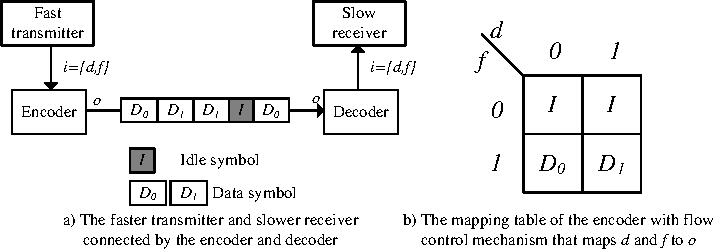
\includegraphics[width=\textwidth]{nonuniq_pred}
\caption{带有流控机制的编码器}
\label{fig_fc}
\end{figure}

\begin{figure}[b]
\centering
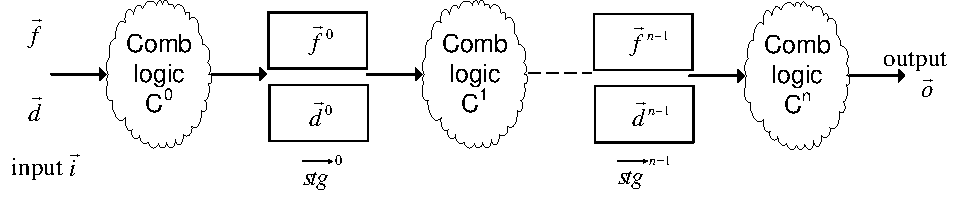
\includegraphics[width=0.9\textwidth]{pipemod1_pred}
\caption{带有流水线和流控机制的编码器}
\label{fig_pipeenc}
\end{figure}



另一方面,
如图\ref{fig_pipeenc}所示,
许多编码器
包含流水线级$\vec{stg}^j$ 以将关键的数据路径划分为多个子段$C^j$,
以提高运行频率。
类似于$\vec{i}$,
每个流水线级$\vec{stg}^j$ 也可以划分为流控向量$\vec{f}^j$ 和数据向量$\vec{d}^j$。

Qin et al. \upcite{QinTODAES15} 首次提出了能够处理流控机制的对偶综合算法。
该算法首先找到所有的能够被$\vec{o}$唯一决定的$i\in\vec{f}$。
然后推导一个能使得$\vec{d}$ 被$\vec{o}$唯一决定的谓词$valid(\vec{f})$。

然而Qin et al. 的算法\upcite{QinTODAES15}在处理流控机制的同时,
却无法处理流水线结构。
这导致其产生的解码器不包含流水线,
并进而使得其运行频率远低于相应的编码器。
为了解决该问题,
本文提出了一个全新的算法,
以为此类同时包含流控机制和流水线的编码器,
产生同样带有流控和流水线的解码器。
该算法首先使用Qin et al. \upcite{QinTODAES15}的算法来寻找流控向量$\vec{f}$ 并推导流控谓词$valid(\vec{f})$。
然后分别通过强制和不强制$valid(\vec{f})$,
以从所有状态变量集合中找到每一个流水线级$\vec{stg}^j$的数据向量$\vec{d}^j$ 和流控向量$\vec{f}^j$。
最后通过Jiang et al. \upcite{InterpBoolFunction}的算法特征化$\vec{stg}^j$ 和$\vec{i}$的布尔函数。

为了展示该算法的有效性,
我们在多个复杂的工业界实际编码器,
如PCI Express \upcite{pcie} 和以太网\upcite{IEEE8023_S4},
上进行了实验。
实验结果表明,
该算法能够为多个工业界的真实编码器正确的产生带有流控和流水线的解码器,
且时序性能相对于传统的对偶综合算法产生的非流水解码器有巨大的提升。



本文剩余部分如下组织。
%小节\ref{sec_prem} 介绍相关的背景知识;
小节\ref{sec_framework} 介绍本文算法的整体结构;
小节\ref{sec_pipeinfer} 找到每一个流水线级$\vec{stg}^j$中的$\vec{f}^j$ 和$\vec{d}^j$ 。
小节\ref{sec_char_chap6} 为$\vec{stg}^j$ 和$\vec{i}$特征化布尔函数。
小节\ref{sec_exp} 和\ref{sec_conclude} 分别给出实验结果和结论。


%
%\section{背景知识}\label{sec_prem}
%
%% \subsection{Flow control mechanism}\label{subsec_fc}
%
%
%
%\subsection{命题逻辑可满足}\label{subsec_SAT}
%布尔集合记为$\mathbb{B}=\{0,1\}$。
%多个变量组成的向量记为$\vec{v}=(v,\dots)$。
%$\vec{v}$ 中的变量个数记为$|\vec{v}|$。
%若一个变量$v$ 是$\vec{v}$的成员,
%则记为$v\in\vec{v}$;
%否则记为$v\notin\vec{v}$。
%对于一个变量$v$ 和一个向量$\vec{v}$,
%若$v\notin\vec{v}$,
%则一个同时包含$v$ 和所有$\vec{v}$ 的成员的新变量记为$v\cup\vec{v}$。
%若$v\in \vec{v}$,
%则一个包含$\vec{v}$ 的所有成员,但是不包含$v$的
%新变量记为$\vec{v}-v$。
%对于两个向量$\vec{a}$ 和$\vec{b}$,
%则同时包含$\vec{a}$ 和$\vec{b}$ 的所有成员的新向量记为$\vec{a}\cup\vec{b}$。
%
%对于变量集合$V$上的公式$F$,
%其命题逻辑可满足问题(SAT)
%的目的在于巡展赋值函数$A:V\to \mathbb{B}$,
%使得$F$ 能够取值为$1$。
%若$A$ 存在则$F$ 是可满足的;
%否则是不可满足的。
%
%对于两个布尔命题逻辑公式$\phi_A$ 和$\phi_B$,
%若$\phi_A\wedge \phi_B$ 不可满足,
%则存在仅引用$\phi_A$ 和$\phi_B$共同变量的公式$\phi_I$ ,
%使得$\phi_A\Rightarrow \phi_I$
%且$\phi_I\wedge \phi_B$ 不可满足。
%$\phi_I$ 称为$\phi_A$ 相对于$\phi_B$的Craig 插值\cite{Craig} 。
%可以使用McMillan算法 \cite{interp_McMillan} 产生该插值。
%
%
%
%
%\subsection{有限状态机}\label{subsec_fsm}
%
%
%
%编码器使用有限状态机$M=(\vec{s},\vec{i},\vec{o},T)$作为模型,
%其中包含状态向量$\vec{s}$。
%输入向量$\vec{i}$,
%输出向量$\vec{o}$,
%状态迁移函数$T: \vec{s}\times \vec{i}\to \vec{s}\times \vec{o}$
%从当前状态向量和输入向量计算出下一状态向量和输出向量。
%
%$M$ 的行为可以通过展开状态迁移函数进行推导。
%状态变量$s\in\vec{s}$, 输入变量$i\in\vec{i}$ 和输出变量$o\in\vec{o}$ 在上述展开序列的第$n$步中
%分别记为$s_n$, $i_n$ 和$o_n$。
%更进一步的,
%在第$n$步中的状态向量,输入向量和输出向量分别记为$\vec{s}_n$, $\vec{i}_n$ 和$\vec{o}_n$。
%一个路径是一个序列$<\vec{s}_n,\dots,\vec{s}_m>$ 使得对于所有$n\le j< m$,
%有$\exists \vec{i}_j\vec{o}_j (\vec{s}_{j+1},\vec{o}_j)\equiv T(\vec{s}_j,\vec{i}_j)$ 。
%而一个环是一个路径$<\vec{s}_n,\dots,\vec{s}_m>$ 使得$\vec{s}_n\equiv \vec{s}_m$。
%
%
%
%\subsection{寻找$\vec{f}$的停机算法}\label{subsec_chkextdec}
%
%
%秦et al. \cite{QinTODAES15} 提出了一个寻找$\vec{f}$ 的停机算法。
%该算法通过迭代的调用一个sound和一个complete的算法以最终得到收敛的答案。.
%% The first one is an under-approximative one that presented in \ref{subsub_sound},
%% while the second one is an over-approximative one presented in \ref{subsub_complete}.
%% We will present these two approaches below and show
%% that they will eventually converge.
%
%\subsubsection{sound算法}\label{subsub_sound}
%如图\ref{fig_pc}a)所示,
%在展开的迁移关系上,
%一个输入变量$i\in\vec{i}$ 能够被唯一决定,
%是指存在$p$, $l$ 和$r$,
%使得对于输出序列$<\vec{o}_p,\dots,\vec{o}_{p+l+r}>$的每一个取值,
%$i_{p+l}$ 不能同时为0和1。
%折等价于公式(\ref{uniqt1})中的$F_{PC}(p,l,r)$的不可满足性。
%行1 对应于图\ref{fig_pc}a)中的路径,
%而行2 是其拷贝
%行3 强制这两个路径的输出相等。
%而行4 强制$i_{p+l}$ 不等。
%该算法是sound的因为当(\ref{uniqt1}) 不可满足
%$i$ 肯定是$\vec{f}$的成员。
%
%\begin{equation}\label{uniqt1}
%% \begin{split}
%F_{PC}(p,l,r):=
%\left\{
%\begin{array}{cc}
%&\bigwedge_{m=0}^{p+l+r}
%\{
%(\vec{s}_{m+1},\vec{o}_m)\equiv T(\vec{s}_m,\vec{i}_m)
%\}
%\\
%\wedge&\bigwedge_{m=0}^{p+l+r}
%\{
%(\vec{s'}_{m+1},\vec{o'}_m)\equiv T(\vec{s'}_m,\vec{i'}_m)
%\}
%\\
%\wedge&\bigwedge_{m=p}^{p+l+r}\vec{o}_m\equiv \vec{o'}_m \\
%\wedge& i_{p+l}\equiv 1 \wedge  i'_{p+l}\equiv 0
%% \wedge&\bigwedge_{m=0}^{p+l+r}assertion(\vec{i}_m) \\
%% \wedge&\bigwedge_{m=0}^{p+l+r}assertion(\vec{i'}_m)
%\end{array}
%\right\}
%% \end{split}
%\end{equation}
%
%\begin{figure}[t]
%\begin{center}
%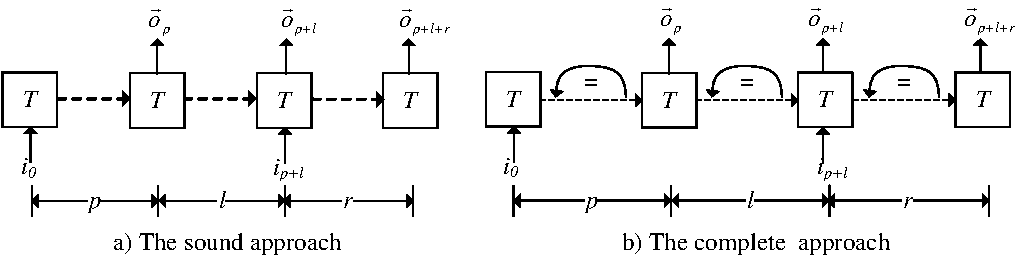
\includegraphics[width=\textwidth]{pc}
%\end{center}
%\caption{sound和complete方法}
%  \label{fig_pc}
%\end{figure}
%
%
%%
%
%
%
%\subsubsection{complete算法}\label{subsub_complete}
%对于上述的$F_{PC}(p,l,r)$ ,
%有两种可能性:
%\textbf{(1)}. 存在$p$, $l$ 和$r$,使得$i_{p+l}$ 能够被$<\vec{o}_{p},\dots,\vec{o}_{p+l+r}>$ 唯一决定;
%或者\textbf{(2)}. $i_{p+l}$ 对于任意$p$, $l$ 和$r$都不能被唯一决定。
%
%
%对于第一种情形,
%通过迭代的增加$p$, $l$ 和$r$,
%$F_{PC}(p,l,r)$ 总能够变成不可满足。
%而对于第二种情形,
%该算法将永不停机。
%因此,
%为了得到一个停机算法,
%我们需要如图\ref{fig_pc}b) 所示的方法去检查第二种情形。
%该方法类似于\ref{fig_pc}a) ,
%但是在三个状态序列$<\vec{s}_{0},\dots,\vec{s}_{p}>$, $<\vec{s}_{p+1},\dots,\vec{s}_{p+l}>$ 和
%$<\vec{s}_{p+l+1},\dots,\vec{s}_{p+l+r}>$上增加了三个约束用于检测环。
%该方法形式化的定义于公式(\ref{uniqln})中。
%其中最后三行即为我们新加的三个约束。
%该方法是complete,
%因为当其是可满足的时候,
%我们可以通过展开
%这三个环来证明第二种情形并断定 $i\notin \vec{f}$。
%
%\begin{equation}\label{uniqln}
%% \begin{split}
%F_{LN}(p,l,r):=\\
%\left\{
%\begin{array}{cc}
%&F_{PC}(p,l,r)\\
%\wedge&\bigvee_{x=0}^{p-1}\bigvee_{y=x+1}^{p} \{\vec{s}_x\equiv \vec{s}_y\wedge \vec{s'}_x\equiv \vec{s'}_y\} \\
%\wedge&\bigvee_{x=p+1}^{p+l-1}\bigvee_{y=x+1}^{p+l} \{\vec{s}_x\equiv \vec{s}_y\wedge \vec{s'}_x\equiv \vec{s'}_y\} \\
%\wedge&\bigvee_{x=p+l+1}^{p+l+r-1}\bigvee_{y=x+1}^{p+l+r} \{\vec{s}_x\equiv \vec{s}_y\wedge \vec{s'}_x\equiv \vec{s'}_y\}
%\end{array}
%\right\}
%% \end{split}
%\end{equation}
%
%
%\subsubsection{通过算法\ref{alg_fofc}找到$\vec{f}$ }\label{subsubsec_findfc}
%
%在行\ref{adduniq},
%所有能够被唯一决定的输入$i$ 将被移到$\vec{f}$。
%若$F_{LN}(p,l,r)$ 在行\ref{nonuniqres}是可满足的,
%所有可满足的输入$i$ 将被移到$\vec{d}$.
%该算法的正确性和停机性证明请见\cite{QinTODAES15} 。
%
%\begin{algorithm}[t]
%\begin{algorithmic}[1]
%\STATE{输入:输入向量$\vec{i}$.}
%\STATE{输出:$\vec{f}\subset \vec{i}$, 在此次搜索中找到的最大$p$, $l$ 和$r$ }
%\STATE $\vec{f}: = \{\}$;$\vec{d}:= \{\}$;$p$:= 0 ;~$l$:= 0 ;~$r$:= 0 \;
%\label{while}\WHILE{$\vec{i}\ne \{\}$}
%  \STATE 假设$i\in\vec{i}$\;
%  \STATE $p++$; ~ $l++$; ~ $r++$\;
%  \IF {$F_{PC}(p,l,r)$ 对于$i$不可满足}
%    \label{adduniq}
%    \STATE $\vec{f}:= i\cup\vec{f}$ ; ~
%    \STATE $\vec{i}:=\vec{i}-i$\;
%  \label{nonuniqres}
%  \ELSIF {$F_{LN}(p,l,r)$ 对于$i$可满足}
%    \STATE $\vec{d}:=i\cup\vec{d}$ ; ~
%    \STATE $\vec{i}:=\vec{i}-i$
%  \ENDIF
%\ENDWHILE
%\RETURN ($\vec{f}$, $p$, $l$, $r$)
%\caption{Identifying the flow control vector $\vec{f}$}
%\label{alg_fofc}
%\end{algorithmic}
%\end{algorithm}
%
%
%
%
%
%\subsection{推导使得$\vec{d}$ 被唯一决定的$valid(\vec{f})$ }\label{subsec_infer}
%
%该算法也是由秦et al. \cite{QinTODAES15}提出的。
%它首先给出算法\ref{alg_craigchar},
%该算法用于特征化一个函数,覆盖所有能够使得一个布尔关系满足的赋值集合。
%然后如图\ref{fig_mono}所示,
%算法\ref{alg_craigchar} 被用于特征化函数$\neg FSAT_{PC}(p,l,r)$,
%$valid(\vec{f})$的单调递增下估计,
%和$\neg FSAT_{LN}(p,l,r)$,
%$valid(\vec{f})$的单调递减上估计。
%最终我们指出这两者将收敛到$valid(\vec{f})$。
%% Please refer to \cite{QinTODAES15} for the proof of its correctness and termination.
%
%
%
%\subsubsection{特征化使得一个布尔关系可满足的布尔函数}\label{subsubsec_craig}
%
%对于一个布尔关系$R(\vec{a},\vec{b},t)$,
%有$R(\vec{a},\vec{b},0)\wedge R(\vec{a},\vec{b},1)$ 不可满足。
%算法\ref{alg_craigchar} 特征化一个布尔寒素$FSAT_R(\vec{a})$,
%该函数覆盖且仅覆盖了能使得
%$R(\vec{a},\vec{b},1)$ 可满足的所有$\vec{a}$。
%行\ref{testsat} 找到$\vec{a}$ 的一个赋值,
%尚未被 $FSAT_R(\vec{a})$ 覆盖而且能够使得$R(\vec{a},\vec{b},1)$ 可满足。
%行\ref{cofact1}, \ref{cofact2} 和\ref{ab} 使用
%McMillan算法\cite{interp_McMillan} 将该赋值放大为$ITP(\vec{a})$。
%行\ref{add} 将$ITP(\vec{a})$ 加入$FSAT_R(\vec{a})$。
%
%
%\begin{algorithm}[t]
%\begin{algorithmic}[1]
%\STATE{输入:布尔关系$R(\vec{a},\vec{b},t)$}
%\STATE{输出:能够使得$R(\vec{a},\vec{b},1)$ 可满足的$FSAT_R(\vec{a})$ }
%\label{initcondition}
%\STATE $FSAT_R(\vec{a}):= 0$ ;
%\label{testsat}
%\WHILE { $R(\vec{a},\vec{b},1)\wedge\neg FSAT_R(\vec{a})$ 可满足}
%  \STATE 假设$A:\vec{a}\cup\vec{b}\cup\{t\}\rightarrow \{0,1\}$ 是一个可满足赋值;
%\label{cofact1}
%  \STATE $\phi_A(\vec{a}):= R(\vec{a},A(\vec{b}),1)$ ;
%\label{cofact2}
%  \STATE $\phi_B(\vec{a}):= R(\vec{a},A(\vec{b}),0)$ ;
%\label{ab}
%  \STATE 假设$ITP(\vec{a})$ 是$\phi_A$ 相对于$\phi_B$ 的Craig插值 ;
%\label{add}
%  \STATE $FSAT_R(\vec{a}):= ITP(\vec{a}) \vee FSAT_R(\vec{a})$ ;
%\ENDWHILE
%\RETURN $FSAT_R(\vec{a})$
%\caption{$CharacterizingFormulaSAT(R,\vec{a},\vec{b},t)$}
%\label{alg_craigchar}
%\end{algorithmic}
%\end{algorithm}
%
%\subsubsection{计算$valid(\vec{f})$的单调递增下估计}\label{subsub_nonloop}
%通过将公式(\ref{uniqt1}) 中的$i$替换为算法\ref{alg_fofc}中推导的$\vec{d}$ ,
%我们有:
%
%\begin{equation}\label{uniqt1d}
%% \begin{split}
%F^d_{PC}(p,l,r):=
%\left\{
%\begin{array}{cc}
%&\bigwedge_{m=0}^{p+l+r}
%\{
%(\vec{s}_{m+1},\vec{o}_m)\equiv T(\vec{s}_m,\vec{i}_m)
%\}
%\\
%\wedge&\bigwedge_{m=0}^{p+l+r}
%\{
%(\vec{s'}_{m+1},\vec{o'}_m)\equiv T(\vec{s'}_m,\vec{i'}_m)
%\}
%\\
%\wedge&\bigwedge_{m=p}^{p+l+r}\vec{o}_m\equiv \vec{o'}_m \\
%\wedge& \vec{d}_{p+l}\ne \vec{d}'_{p+l} \\
%% \wedge&\bigwedge_{m=0}^{p+l+r}assertion(\vec{i}_m) \\
%% \wedge&\bigwedge_{m=0}^{p+l+r}assertion(\vec{i'}_m)
%\end{array}
%\right\}
%% \end{split}
%\end{equation}
%
%% Here,
%% $\vec{d}_{p+l}\ne \vec{d}'_{p+l}$ means some bit in $\vec{d}_{p+l}$
%% isn't equal to the corresponding bit in $\vec{d}'_{p+l}$.
%若$F^d_{PC}(p,l,r)$ 可满足,
%则$\vec{d}_{p+l}$ 不能被$<\vec{o}_p,\dots,\vec{o}_{p+l+r}>$唯一决定。
%通过收集公式 (\ref{uniqt1d})的第三行,
%我们定义$T_{PC}(p,l,r)$ :
%
%\begin{equation}\label{tpc}
%% \begin{split}
%T_{PC}(p,l,r):=\\
%\left\{
%\begin{array}{cc}
%      &\bigwedge_{m=p}^{p+l+r}\vec{o}_m\equiv \vec{o'}_m \\
%\end{array}
%\right\}
%% \end{split}
%\end{equation}
%
%\begin{figure}[b]
%\begin{center}
%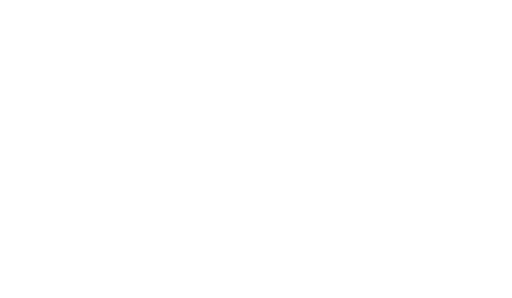
\includegraphics[width=0.5\textwidth]{mono}
%\end{center}
%\caption{The monotonicity of $FSAT_{PC}(p,l,r)$ and $FSAT_{LN}(p,l,r)$}
%  \label{fig_mono}
%\end{figure}
%
%通过将$T_{PC}(p,l,r)$ 替换回$F^d_{PC}(p,l,r)$,
%我们有:
%
%\begin{equation}\label{fpcq}
%% \begin{split}
%F'^d_{PC}(p,l,r,t):=
%\left\{
%\begin{array}{cc}
%&\bigwedge_{m=0}^{p+l+r}
%\{
%(\vec{s}_{m+1},\vec{o}_m)\equiv T(\vec{s}_m,\vec{i}_m)
%\}
%\\
%\wedge&\bigwedge_{m=0}^{p+l+r}
%\{
%(\vec{s'}_{m+1},\vec{o'}_m)\equiv T(\vec{s'}_m,\vec{i'}_m)
%\}
%\\
%\wedge& t\equiv T_{PC}(p,l,r)\\
%\wedge& \vec{d}_{p+l}\ne \vec{d'}_{p+l} \\
%% \wedge&\bigwedge_{m=0}^{p+l+r}assertion(\vec{i}_m) \\
%% \wedge&\bigwedge_{m=0}^{p+l+r}assertion(\vec{i'}_m)
%\end{array}
%\right\}
%% \end{split}
%\end{equation}
%
%
%很明显$F^d_{PC}(p,l,r)$ 和$F'^d_{PC}(p,l,r,1)$ 是等价的,
%我们进一步定义:
%
%\begin{equation}\label{pcdef1}
%\vec{a}:=\vec{f}_{p+l}
%\end{equation}
%
%\begin{equation}\label{pcdef2}
%\vec{b}:=\vec{d}_{p+l}\cup \vec{d'}_{p+l}\cup \vec{s}_0\cup \vec{s'}_0\cup\bigcup_{0\le x\le p+l+r,x\neq (p+l)}(\vec{i}_{x}\cup\vec{i'}_{x})
%\end{equation}
%
%因此,
%向量$\vec{a}\cup\vec{b}$ 包含所有步的输入向量$<\vec{i}_0,\dots,\vec{i}_{p+l+r}>$ 和$<\vec{i'}_0,\dots,\vec{i'}_{p+l+r}>$。
%它同时也包含两个初始状态$\vec{s}_0$ 和$\vec{s'}_0$。
%因此$\vec{a}$ 和$\vec{b}$ 能唯一决定$F'^d_{PC}(p,l,r,t)$中$t$ 的取值。
%这意味着$R(\vec{a},\vec{b},1)\wedge R(\vec{a},\vec{b},0)$ 是不可满足的。
%因此,
%对于$p$, $l$ 和$r$的特定组合,
%在$\vec{f}_{p+l}$ 上定义且能够使$F'^d_{PC}(p,l,r,1)$ 满足的函数可以通过使用$F'^d_{PC}(p,l,r,t)$, $\vec{a}$ 和$\vec{b}$ 调用算法定义如下:
%
%\begin{equation}\label{fsat_pc}
%FSAT_{PC}(p,l,r):=CharacterizingFormulaSAT(F'^d_{PC}(p,l,r,t),\vec{a},\vec{b},t)
%\end{equation}
%
%如图\ref{fig_mono}所示,
%$\neg FSAT_{PC}(p,l,r)$ 是$valid(\vec{f})$ 的针对
%$p$, $l$ 和$r$
%单调递增的下估计。
%% \end{proposition}
%
%
%
%
%\subsubsection{计算$valid(\vec{f})$的单调递减上估计}\label{subsub_loop}
%类似的,
%我们定义:
%
%\begin{equation}\label{tln}
%% \begin{split}
%T_{LN}(p,l,r):=\\
%\left\{
%\begin{array}{cc}
%      &\bigwedge_{m=p}^{p+l+r}\vec{o}_m\equiv \vec{o'}_m \\
%\wedge&\bigvee_{x=0}^{p-1}\bigvee_{y=x+1}^{p} \{\vec{s}_x\equiv \vec{s}_y\wedge \vec{s'}_x\equiv \vec{s'}_y\} \\
%\wedge&\bigvee_{x=p+1}^{p+l-1}\bigvee_{y=x+1}^{p+l} \{\vec{s}_x\equiv \vec{s}_y\wedge \vec{s'}_x\equiv \vec{s'}_y\} \\
%\wedge&\bigvee_{x=p+l+1}^{p+l+r-1}\bigvee_{y=x+1}^{p+l+r} \{\vec{s}_x\equiv \vec{s}_y\wedge \vec{s'}_x\equiv \vec{s'}_y\}
%\end{array}
%\right\}
%% \end{split}
%\end{equation}
%
%
%
%\begin{equation}\label{lndef1}
%F'^d_{LN}(p,l,r,t):=
%\left\{
%\begin{array}{cc}
%&\bigwedge_{m=0}^{p+l+r}
%\{
%(\vec{s}_{m+1},\vec{o}_m)\equiv T(\vec{s}_m,\vec{i}_m)
%\}
%\\
%\wedge&\bigwedge_{m=0}^{p+l+r}
%\{
%(\vec{s'}_{m+1},\vec{o'}_m)\equiv T(\vec{s'}_m,\vec{i'}_m)
%\}
%\\
%% \wedge& \vec{f}_{p+l}\equiv \vec{f'}_{p+l}\\
%\wedge& t\equiv T_{LN}(p,l,r)\\
%\wedge& \vec{d}_{p+l}\ne \vec{d'}_{p+l} \\
%% \wedge&\bigwedge_{m=0}^{p+l+r}assertion(\vec{i}_m) \\
%% \wedge&\bigwedge_{m=0}^{p+l+r}assertion(\vec{i'}_m)
%\end{array}
%\right\}
%\end{equation}
%
%
%\begin{equation}\label{fsat_ln}
%FSAT_{LN}(p,l,r):=CharacterizingFormulaSAT(F'^d_{LN}(p,l,r,t),\vec{a},\vec{b},t)
%\end{equation}
%
%如图\ref{fig_mono}所示,
%$\neg FSAT_{LN}(p,l,r)$ 是$valid(\vec{f})$ 相对于$p$, $l$ 和$r$.的一个单调递减的上估计。
%
%
%
%\subsubsection{使用算法\ref{algo_infer}推导$valid(\vec{f})$ }\label{subsub_overal}
%\begin{algorithm}[t]
%\begin{algorithmic}[1]
%\STATE $p$:= $0$;~$l$:= $0$;~$r$:= $0$ \;
%\WHILE{ $\neg FSAT_{LN}(p,l,r)\wedge FSAT_{PC}(p,l,r)$ 可满足}
%  \STATE $p$ ++ ;~$l$ ++ ;~$r$ ++ ;
%\ENDWHILE
%\RETURN {$\neg FSAT_{LN}(p,l,r)$}
%\caption{推导$valid(\vec{f}_{p+l})$}
%\label{algo_infer}
%\end{algorithmic}
%\end{algorithm}
%
%该算法迭代的增加$p$, $l$ 和$r$,
%直到$FSAT_{PC}(p,l,r)$ 和$FSAT_{LN}(p,l,r)$ 收敛。
%其正确性和停机性见\cite{QinTODAES15} 。


\section{算法框架}\label{sec_framework}


\subsection{编码器的一般性模型}
如图\ref{fig_pipeenc}所示,
我们假设编码器包含$n$个流水线级$\vec{stg}^j$,
其中$0\le j \le n-1$。
和上一章的图\ref{fig_pipeenc_chap4}不同的是,
每一个流水线级$\vec{stg}^j$ 能够被进一步划分为流控向量$\vec{f}^j$ 和数据向量$\vec{d}^j$。
而输入向量$\vec{i}$,
和Qin et al.\upcite{QinTODAES15}一样,
也能被划分为流控向量$\vec{f}$ 和数据向量$\vec{d}$。
如果将组合逻辑块$C^j$ 视为一个函数,
则该编码器可以使用下列等式定义:

\begin{equation}\label{equ_genpipe}
\begin{array}{cccc}
\vec{stg}^0   & := & C^0(\vec{i})         &\\
\vec{stg}^j   & := & C^j(\vec{stg}^{j-1}) & 1\le j\le n-1\\
\vec{o}       & := & C^n(\vec{stg}^{n-1}) &
\end{array}
\end{equation}


%\begin{figure}[b]
%\begin{center}
%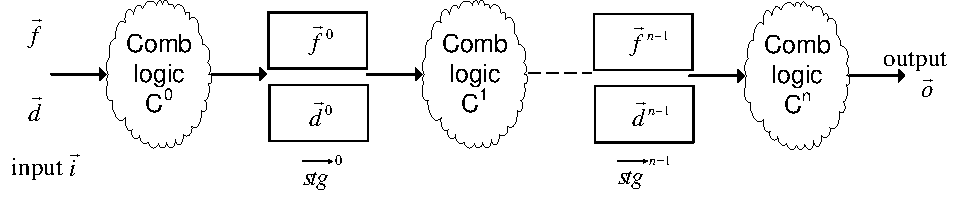
\includegraphics[width=\textwidth]{pipemod1_pred}
%\end{center}
%\caption{包含流水线级和流控机制的一般性编码器模型}
%  \label{fig_pipeenc}
%\end{figure}



在本文中,
上标始终意味着流水线级,
而下标,
如小节\ref{subsec_fsm}指出,
始终意味着在展开的迁移关系序列中的步。
例如,
$\vec{stg}^j$ 是第$j$个流水线级。
而$\vec{stg}^j_k$ 是该第$j$流水线级
在第$k$步的取值。

\subsection{算法框架}\label{algo_algoframework}

基于图\ref{fig_pipeenc}所示的编码器结构,
我们算法的框架为:

\begin{enumerate}
 \item 调用算法\ref{alg_fofc} 以将$\vec{i}$ 划分为$\vec{f}$ 和$\vec{d}$。
 \item 调用算法\ref{algo_infer} 以推导能够使得$\vec{d}$
 被唯一决定的$valid(\vec{f})$和其对应的$p$, $l$ 和$r$。
 \item 在小节\ref{sec_pipeinfer},
 找到每一个流水线级$\vec{stg}^j$中的$\vec{f}^j$ 和$\vec{d}^j$ 。
 \item 在小节\ref{sec_char_chap6}中特征化每一个流水线级$\vec{stg}^j$和输入$\vec{i}$的布尔函数,
 即图\ref{fig_pipeenc}中每一个组合逻辑函数$C^j$的反$(C^j)^{-1}$,
 以构造最终的解码器。
\end{enumerate}



\section{推导流水线结构}\label{sec_pipeinfer}


\subsection{压缩$r$ 和$l$}\label{reduceing}

\begin{algorithm}[b]
\begin{algorithmic}[1]
\FOR{$r':=r \to 0$}
\label{testr_1}
  \IF{$r'\equiv 0$ or $F_{PC}(p,l,r'-1)\wedge valid(\vec{f}_{p+l})\wedge valid(\vec{f'}_{p+l})$ 对于某些$i\in \vec{i}$可满足}
    \STATE break
  \ENDIF
\ENDFOR
\RETURN $r'$
\caption{压缩$r$}
\label{algo_remove2}
\end{algorithmic}
\end{algorithm}

由于算法\ref{algo_infer} 同时增加$p$, $l$ 和$r$ ,
因此$l$ 和$r$存在一定程度的冗余。
因此我们需要首先在算法\ref{algo_remove2}中压缩$r$。


在行\ref{testr_1},
我们将推导的谓词$valid(\vec{f})$ 和$F_{PC}(p,l,r'-1)$与在一起。
当该公式可满足时,
则$r'$ 是最后一个使得$F_{PC}(p,l,r')\wedge valid(\vec{f}_{p+l})\wedge valid(\vec{f'}_{p+l})$ 不可满足的值,
我们将其直接直接返回。
另一方面,
当$r'\equiv 0$,
$F_{PC}(p,l,0)$ 肯定已经在上一个迭代中被测试,
且结果为不可满足。
此时我们直接返回$0$。


这样,
我们从算法\ref{algo_remove2}得到了一个压缩的$r$,
使得$\vec{i}_{p+l}$ 可以被$<\vec{o}_{p},\dots,\vec{o}_{p+l+r}>$唯一决定。

\begin{figure}[t]
\begin{center}
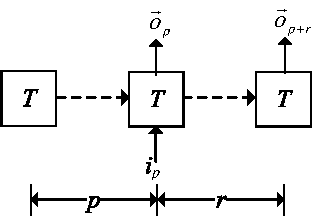
\includegraphics[width=0.5\textwidth]{pc1_pred}
\end{center}
\caption{使用削减的输出序列恢复输入}
  \label{fig_pc1}
\end{figure}

我们进一步要求:
\begin{enumerate}
 \item 如图\ref{fig_pc1}所示,
 $l$ 可以被削减为0。
 这意味着$\vec{i}_{p}$ 可以被$<\vec{o}_{p},\dots,\vec{o}_{p+r}>$唯一决定,
 即所有的未来输出。
 \item 上述的输出序列$<\vec{o}_{p},\dots,\vec{o}_{p+r}>$
 能被进一步压缩为$\vec{o}_{p+r}$。
 这意味着只需$\vec{o}_{p+r}$ 即可唯一决定$\vec{i}_p$。
\end{enumerate}

检验这两个要求等价于
检查$F'_{PC}(p,r)\wedge valid(\vec{f}_{p})\wedge valid(\vec{f'}_{p})$的不可满足性
其中$F'_{PC}(p,r)$ 定义如下:

\begin{equation}\label{uniqt11}
% \begin{split}
F'_{PC}(p,r):=
\left\{
\begin{array}{cc}
&\bigwedge_{m=0}^{p+r}
\{
(\vec{s}_{m+1},\vec{o}_m)\equiv T(\vec{s}_m,\vec{i}_m)
\}
\\
\wedge&\bigwedge_{m=0}^{p+r}
\{
(\vec{s'}_{m+1},\vec{o'}_m)\equiv T(\vec{s'}_m,\vec{i'}_m)
\}
\\
\wedge&\vec{o}_{p+r}\equiv \vec{o'}_{p+r} \\
\wedge& i_{p}\equiv 1 \wedge  i'_{p}\equiv 0\\
\wedge&\bigwedge_{m=0}^{p+r}assertion(\vec{i}_m) \\
\wedge&\bigwedge_{m=0}^{p+r}assertion(\vec{i'}_m)
\end{array}
\right\}
% \end{split}
\end{equation}


该要求看起来远远强于(\ref{uniqt1})。
我们将在实验结果中指出他们总是不可满足的。



\subsection{寻找流控向量$\vec{f}^j$和数据向量$\vec{d}^j$}\label{subsec_inferstage}

现在,
基于上述推导的$p$ 和$r$,
我们将公式(\ref{uniqt11}) 中的$F'_{PC}$推广到下面定义的更广泛的形式。
它能够检查任意变量$v$ 在步$j$
能否被向量$\vec{w}$ 在步$k$唯一决定。
现在$v$ 和$\vec{w}$ 可以使输入,输出或者状态向量。

\begin{equation}\label{uniqt2}
% \begin{split}
F''_{PC}(p,r,v,j,\vec{w},k):=
\left\{
\begin{array}{cc}
&\bigwedge_{m=0}^{p+r}
\{
(\vec{s}_{m+1},\vec{o}_m)\equiv T(\vec{s}_m,\vec{i}_m)
\}
\\
\wedge&\bigwedge_{m=0}^{p+r}
\{
(\vec{s'}_{m+1},\vec{o'}_m)\equiv T(\vec{s'}_m,\vec{i'}_m)
\}
\\
\wedge&\vec{w}_{k}\equiv \vec{w'}_{k} \\
\wedge& v_{j}\equiv 1 \wedge  v'_{j}\equiv 0\\
\wedge&\bigwedge_{m=0}^{p+r}assertion(\vec{i}_m) \\
\wedge&\bigwedge_{m=0}^{p+r}assertion(\vec{i'}_m)
\end{array}
\right\}
% \end{split}
\end{equation}

很明显,
当$F''_{PC}(p,r,v,j,\vec{w},k)\wedge valid(\vec{f}_{p})\wedge valid(\vec{f'}_{p})$ 不可满足时,
$\vec{w}_k$ 能唯一决定$v_j$.

对于$0\le j\le n-1$,
在第$j$流水线级$\vec{stg}^j$,
其流控向量$\vec{f}^j$ 包含所有
能够在第$j-((n-1)-(p+r))$-th 步被$\vec{o}$
在第$p+r$步唯一决定的状态变量$s\in \vec{s}$。
注意在这里不需要约束$valid(\vec{f}_p)$。
这可以形式化的定义为:

\begin{equation}\label{stgn_fj}
\vec{f}^{j} :=
 \left\{
 s\in \vec{s} ~|
\begin{array}{cc}
 F''_{PC}(p,r,s,j-D,\vec{o},p+r)\\
 ~is~unsatisfiable
\end{array}
\right\}
\end{equation}

其中:

\begin{equation}\label{stgn_def}
\begin{array}{ccc}
% S             & := & \vec{s}/\bigcup_{j<k\le n-2}\vec{stg}^{k}\\
D             & := & (n-1)-(p+r)\\
\end{array}
\end{equation}

而在第$j$流水线级$\vec{stg}^j$中的数据向量$\vec{d}^j$
包含能够在第$j-((n-1)-(p+r))$步被
$\vec{o}$ 在第$p+r$步唯一决定的所有$s\in \vec{s}$。
注意这里我们需要强制$valid(\vec{f}_p)$。
这可以被形式化的定义为:

\begin{equation}\label{stgn_dj}
\vec{d}^{j} :=
 \left\{
 s\in \vec{s} ~|
 \begin{array}{cc}
 F''_{PC}(p,r,s,j-D,\vec{o},p+r)\wedge valid(\vec{f}_{p})\wedge valid(\vec{f'}_{p})\\
 ~is~unsatisfiable
 \end{array}
\right\}
\end{equation}


\subsection{推导每一级流水线上的控制流谓词$valid(\vec{f}^j)$}\label{subsec_inferstage}
本节目的在于,
为每一个流水线级$\vec{stg}^j$上的流控向量$\vec{f}^j$,
推导一个使得$\vec{d}^j$能够被唯一决定的谓词$valid(\vec{f}^j)$。

在这里$valid(\vec{f}^j)$的作用类似于输入向量$\vec{i}$上的$valid(\vec{f})$。
其中后者用于表示输入的数据向量$\vec{d}$的有效性。
因此$valid(\vec{f}^j)$被用于表示流水线级$\vec{stg}^j$上的数据向量$\vec{d}^j$的有效性。

在小节\ref{subsub_overal}中,
我们给出了一个迭代的复杂算法\ref{algo_infer}以推导$valid(\vec{f})$。
而在这里,
我们并不需要一个类似的迭代算法,
因为该算法所需要的$p$,$l$和$r$已经在小节\ref{algo_algoframework}的第2步中被算法\ref{algo_infer}推导得到了。

因此,我们在这里可以简单的使用如下算法:

首先构造如下公式:

\begin{equation}\label{uniqt1d_chap6}
% \begin{split}
F^f_{PC}(p,l,r):=
\left\{
\begin{array}{cc}
&\bigwedge_{m=0}^{p+r}
\{
(\vec{s}_{m+1},\vec{o}_m)\equiv T(\vec{s}_m,\vec{i}_m)
\}
\\
\wedge&\bigwedge_{m=0}^{p+r}
\{
(\vec{s'}_{m+1},\vec{o'}_m)\equiv T(\vec{s'}_m,\vec{i'}_m)
\}
\\
\wedge&\vec{o}_{p+r}\equiv \vec{o'}_{p+r} \\
\wedge& \vec{f}^j_{j-D}\equiv \vec{f}'^j_{j-D} \\
\wedge& \vec{d}^j_{j-D}\ne \vec{d}'^j_{j-D} \\
\wedge&\bigwedge_{m=0}^{p+r}assertion(\vec{i}_m) \\
\wedge&\bigwedge_{m=0}^{p+r}assertion(\vec{i'}_m)
\end{array}
\right\}
% \end{split}
\end{equation}

该公式的前两行分别是两个展开的迁移函数序列组成的路径。
第三行约束它们的输出在$p+r$步相等。
第四行约束它们在第j级流水线的流控向量$\vec{f}^j$在第$j-D$步相等。
这里的$D$定义于公式(\ref{stgn_def})。
第五行约束它们在第$j$级流水线的数据向量$\vec{d}^j$在第$j-D$步不等。

如果上述$F^f_{PC}(p,l,r)$ 是可满足的,
则$\vec{d}^j_{j-D}$ 无法被$\vec{o}_{p+r}$唯一决定。
通过收集等式(\ref{uniqt1d_chap6})的第三行,我们得到$T_{PC}(p,l,r)$:

\begin{equation}\label{tpc_chap6}
% \begin{split}
T_{PC}(p,l,r):=\\
\left\{
\begin{array}{cc}
      &\vec{o}_{p+r}\equiv \vec{o'}_{p+r} \\
\end{array}
\right\}
% \end{split}
\end{equation}

通过将$T_{PC}(p,l,r)$ 代入到$F^f_{PC}(p,l,r)$,
我们得到一个新的公式:
\begin{equation}\label{fpcq_chap6}
% \begin{split}
F'^f_{PC}(p,l,r):=
\left\{
\begin{array}{cc}
&\bigwedge_{m=0}^{p+r}
\{
(\vec{s}_{m+1},\vec{o}_m)\equiv T(\vec{s}_m,\vec{i}_m)
\}
\\
\wedge&\bigwedge_{m=0}^{p+r}
\{
(\vec{s'}_{m+1},\vec{o'}_m)\equiv T(\vec{s'}_m,\vec{i'}_m)
\}
\\
\wedge& t\equiv T_{PC}(p,l,r)\\
\wedge& \vec{f}^j_{j-D}\equiv \vec{f}'^j_{j-D} \\
\wedge& \vec{d}^j_{j-D}\ne \vec{d}'^j_{j-D} \\
\wedge&\bigwedge_{m=0}^{p+r}assertion(\vec{i}_m) \\
\wedge&\bigwedge_{m=0}^{p+r}assertion(\vec{i'}_m)
\end{array}
\right\}
% \end{split}
\end{equation}


很明显$F^f_{PC}(p,l,r)$ 和$F'^f_{PC}(p,l,r,1)$ 是等价的。
我们进一步定义:

\begin{equation}\label{pcdef1_chap6}
\vec{a}:=\vec{f}^j_{j-D}
\end{equation}

\begin{equation}\label{pcdef2_chap6}
\vec{b}:=\vec{d}^j_{j-D}\cup \vec{d'}^j_{j-D}\cup \bigcup_{j-D\le i\le p+r}(\vec{i}_{x}\cup\vec{i'}_{x})
\end{equation}

% $\vec{f}_{p+l}$ can be uniquely determined,
% so we do not need to consider $\vec{f'}_{p+l}$.
则$\vec{a}\cup\vec{b}$ 包含了两个迁移函数展开序列上从第$j-D$步开始的所有输入向量$<\vec{i}_{j-D},\dots,\vec{i}_{p+r}>$ and $<\vec{i'}_{j-D},\dots,\vec{i'}_{p+r}>$。
他同时也包含了两个展开序列的在第$j-D$步的状态$\vec{d}^j_{j-D}$ 和 $\vec{d'}^j_{j-D}$。
进一步的,
等式(\ref{fpcq_chap6})前两行的迁移关系$T$
能够从输入序列和初始状态唯一的计算出输出序列。
因此$\vec{a}$ 和$\vec{b}$ 能够唯一决定$F'^f_{PC}(p,l,r,t)$中$t$ 的取值。
因此,
对于特定$p$,$l$ 和$r$,
以$\vec{f}^j_{j-D}$ 为输入并使得$F'^f_{PC}(p,l,r,1)$ 可满足的函数可以通过以$F'^d_{PC}(p,l,r,t)$, $\vec{a}$ 和$\vec{b}$ 为参数调用算法\ref{alg_craigchar}得到:

\begin{equation}\label{fsat_pc_chap6}
FSAT^j_{PC}(p,l,r):=CharacterizingFormulaSAT(F'^f_{PC}(p,l,r,t),\vec{a},\vec{b},t)
\end{equation}

因此$FSAT^j_{PC}(p,l,r)$ 覆盖了
使得$F^f_{PC}(p,l,r)$ 可满足的$\vec{f}^j_{j-D}$赋值集合。
因此,
其反$\neg FSAT^j_{PC}(p,l,r)$ 是使得
$F^f_{PC}(p,l,r)$ 不可满足的$\vec{f}^j_{j-D}$集合。
因此有:

\begin{equation}
valid(\vec{f}^j):=\neg FSAT^j_{PC}(p,l,r)
\end{equation}





\section{特征化流水线级和输入的布尔函数}\label{sec_char_chap6}
\subsection{特征化最后一个流水线级的布尔函数}

从公式(\ref{stgn_fj})可知,
每个状态变量$s\in \vec{f}^{n-1}$ 能够被$\vec{o}$ 在第$p+r$步唯一决定。
也就是,
$F''_{PC}(p,r,s,p+r,\vec{o},p+r)$ 不可满足且可以划分为:

\begin{equation}
 \phi_A :=
 \left\{
\begin{array}{cc}
&\bigwedge_{m=0}^{p+r}
\{
(\vec{s}_{m+1},\vec{o}_m)\equiv T(\vec{s}_m,\vec{i}_m)
\}
\\
\wedge& s_{p+r}\equiv 1 \\
\wedge&\bigwedge_{m=0}^{p+r}assertion(\vec{i}_m) 
\end{array}
\right\}
\end{equation}

\begin{equation}
% \begin{split}
\phi_B :=
\left\{
\begin{array}{cc}
&\bigwedge_{m=0}^{p+r}
\{
(\vec{s'}_{m+1},\vec{o'}_m)\equiv T(\vec{s'}_m,\vec{i'}_m)
\}
\\
\wedge&\vec{o}_{p+r}\equiv \vec{o'}_{p+r} \\
\wedge& s'_{p+r}\equiv 0 \\
\wedge&\bigwedge_{m=0}^{p+r}assertion(\vec{i'}_m)
\end{array}
\right\}
% \end{split}
\end{equation}

因为$F''_{PC}(p,r,s,p+r,\vec{o},p+r)$ 等价于$\phi_A \wedge \phi_B$,
所以$\phi_A \wedge \phi_B$ 不可满足
而$\phi_A$ 和$\phi_B$ 的共同变量集合是$\vec{o}_{p+r}$。

根据文献\upcite{InterpBoolFunction},
$\phi_A$ 相对于$\phi_B$ 的Craig插值$\phi_I$可以被计算出来,
只引用$\vec{o}_{p+r}$,
并且覆盖所有能使$s_{p+r}\equiv 1$的$\vec{o}_{p+r}$ 。
同时,
$\phi_I\wedge \phi_B$ 不可满足。
这意味着$\phi_I$ 并不覆盖任何使得$s_{p+r}\equiv 0$的$\vec{o}_{p+r}$ 。

因此,
$\phi_I$ 可以作为
从$\vec{o}$恢复$s\in \vec{f}^{n-1}$的布尔函数。

通过将$F''_{PC}(p,r,s,p+r,\vec{o},p+r)$ 替换为$F''_{PC}(p,r,s,p+r,\vec{o},p+r)\wedge valid(\vec{f}_p)\wedge valid(\vec{f'}_p)$,
我们可以类似的特征化恢复$s\in\vec{d}^{n-1}$的布尔函数。
注意此时$valid(\vec{f}_p)$应属于$\phi_A$,
而$valid(\vec{f'}_p)$应属于$\phi_B$。

\subsection{特征化恢复其他流水线级的布尔函数}
根据图\ref{fig_pipeenc},
% Similar to last subsection,
$\vec{f}^j$ 在第$j-D$步可以被$\vec{stg}^{j+1}$ 在第$j-D+1$步唯一决定。
因此我们将不可满足公式$F''_{PC}(p,r,s,j-D,\vec{stg}^{j+1},j-D+1)$
划分为下列两个公式:

\begin{equation}
 \phi_A :=
 \left\{
\begin{array}{cc}
&\bigwedge_{m=0}^{p+r}
\{
(\vec{s}_{m+1},\vec{o}_m)\equiv T(\vec{s}_m,\vec{i}_m)
\}
\\
\wedge& s_{j-D}\equiv 1\\
\wedge&\bigwedge_{m=0}^{p+r}assertion(\vec{i}_m) 
\end{array}
\right\}
\end{equation}

\begin{equation}
% \begin{split}
\phi_B :=
\left\{
\begin{array}{cc}
&\bigwedge_{m=0}^{p+r}
\{
(\vec{s'}_{m+1},\vec{o'}_m)\equiv T(\vec{s'}_m,\vec{i'}_m)
\}
\\
\wedge&\vec{stg}^{j+1}_{j-D+1}\equiv \vec{stg'}^{j+1}_{j-D+1} \\
\wedge& s'_{j-D}\equiv 0\\
\wedge&\bigwedge_{m=0}^{p+r}assertion(\vec{i'}_m)
\end{array}
\right\}
% \end{split}
\end{equation}

再一次,
$\phi_A$ 相对于$\phi_B$ 的Craig插值$\phi_I$可以被构造出来,
并用做从$\vec{stg}^{j+1}$恢复$s\in\vec{f}^{j}$的布尔函数。

类似的,
将$F''_{PC}(p,r,s,j-D,\vec{stg}^{j+1},j-D+1)$  替换为
$F''_{PC}(p,r,s,j-D,\vec{stg}^{j+1},j-D+1)\wedge valid(\vec{f}_p)\wedge valid(\vec{f'}_p)$ ,
我们能特征化从$\vec{stg}^{j+1}$恢复$s\in\vec{d}^{j}$的布尔函数。
注意此时$valid(\vec{f}_p)$应属于$\phi_A$,
而$valid(\vec{f'}_p)$应属于$\phi_B$。

\subsection{特征化从第0级流水线恢复输入向量的布尔函数}

根据图\ref{fig_pipeenc},
$\vec{f}$ 在第$p$步能够被$\vec{stg}^0$ 在第$p$步唯一决定。
$F''_{PC}(p,r,i,p,\vec{stg}^0,p)$ 不可满足并可以划分为以下两个公式:

\begin{equation}
% \begin{split}
\phi_A:=
\left\{
\begin{array}{cc}
&\bigwedge_{m=0}^{p+r}
\{
(\vec{s}_{m+1},\vec{o}_m)\equiv T(\vec{s}_m,\vec{i}_m)
\}
\\
\wedge& i_{p}\equiv 1\\
\wedge&\bigwedge_{m=0}^{p+r}assertion(\vec{i}_m) 
\end{array}
\right\}
% \end{split}
\end{equation}

\begin{equation}
% \begin{split}
\phi_B:=
\left\{
\begin{array}{cc}
&\bigwedge_{m=0}^{p+r}
\{
(\vec{s'}_{m+1},\vec{o'}_m)\equiv T(\vec{s'}_m,\vec{i'}_m)
\}
\\
\wedge&\vec{stg}^0_p\equiv \vec{stg'}^0_p \\
\wedge& i'_{p}\equiv 0\\
\wedge&\bigwedge_{m=0}^{p+r}assertion(\vec{i'}_m)
\end{array}
\right\}
% \end{split}
\end{equation}

再一次,
$\phi_A$ 相对于$\phi_B$的Craig插值$\phi_I$
可以被用作从$\vec{stg}^0$恢复$i\in\vec{f}$的布尔函数。

类似的,
通过替换$F''_{PC}(p,r,i,p,\vec{stg}^0,p)$ 为$F''_{PC}(p,r,i,p,\vec{stg}^0,p)\wedge valid(\vec{f}_p)\wedge valid(\vec{f'}_p)$,
我们可以特征化从$\vec{stg}^0$恢复$i\in\vec{d}$的布尔函数。
注意此时$valid(\vec{f}_p)$应属于$\phi_A$,
而$valid(\vec{f'}_p)$应属于$\phi_B$。


\section{实验结果}\label{sec_exp}
我们使用OCaml 语言\upcite{OCaml}实现了上述算法,
并使用MiniSat 1.14 \upcite{EXTSAT}求解产生的CNF公式。
所有的实验使用一台包含16 个Intel Xeon E5648 2.67GHz处理器,
192GB 内存, 和CentOS 5.4 Linux操作系统的服务器上。

\subsection{比较时间和面积}
表\ref{tab_bench} 给出本文中使用的测试电路。
第2和3列分别给出输入,输出和状态变量个数。
第4列给出了将编码器映射至LSI10K 库所得到的面积。
本文中,
所有的面积和延迟均使用同样的设置得到。


\begin{table*}[t]
\caption{Benchmark和实验结果}
\begin{tabular}{|c|c|c|c|c|c|c|c|c|c|c|}
\hline
 Names     & \multicolumn{4}{|c|}{编码器}                                        &   \multicolumn{3}{|c|}{\cite{ShenTCAD11}产生}      &   \multicolumn{3}{|c|}{本文产生} \\
           & \multicolumn{4}{|c|}{}                                              &   \multicolumn{3}{|c|}{的解码器}                   &   \multicolumn{3}{|c|}{的解码器} \\\cline{2-11}
           &    \#in &   \#    &面积  & 解码器                                   &运行 &延迟 &面积                                    &运行 &延迟 &面积\\
           &   /out  &  reg    &      &   描述                                   &时间 &(ns) &                                        &时间 &(ns) &    \\\hline\hline
 pcie      & 10/11   & 23      & 326  &PCIE                                      &0.37 &7.20 &624                                     &8.08 & 5.89&652 \\
           &         &         &      &     2.0 \upcite{pcie}                    &     &     &                                        &     &     &    \\\hline
 xgxs      & 10/10   & 16      & 453  &     以太网                               &0.21 &7.02 &540                                     &4.25 & 5.93&829 \\
           &         &         &      &              clause 48 \upcite{IEEE8023_S4}&     &     &                                        &     &     &    \\\hline
 t2eth     & 14/14   & 49      & 2252 &    以太网                                &12.7 &6.54 &434                                     &430.4& 6.12&877 \\
           &         &         &      &             clause 36 \upcite{IEEE8023_S4} &     &     &                                        &     &     &    \\\hline
scrambler  &64/64    & 58      & 1034 & inserting                                &     \multicolumn{6}{|c|}{}\\
           &         &         &      &           01 flipping                    &     \multicolumn{6}{|c|}{没有发现 }\\\cline{1-5}
 xfi       & 72/66   & 72      & 7772 &     以太网                               &     \multicolumn{6}{|c|}{流水线级}\\
           &         &         &      &              clause 49 \upcite{IEEE8023_S4}&     \multicolumn{6}{|c|}{}\\\hline
\end{tabular}\label{tab_bench}
\end{table*}





第6到8列分别给出了论文\upcite{ShenTCAD11}的算法产生非流水解码器的运行时间,
以及该解码器的延迟和面积。
而第9到11列分别给出了本文算法的类似信息。

比较第7和10列可知
延迟得到了明显的改善。

一个比较令人惊讶的事实是,
两个最大的测试电路 scrambler 和xfi 并不包含流水线。
我们研究并确认了这一点。
他们的面积如此之大是因为使用了很宽的64到72 位数据路径。

在下面各个小节中,
我们分别给出针对各个测试电路推导出来的流水线结构。

\subsection{针对PCIE推导的流水线结构}

对于pcie,
存在两个流水线级,
其中包含的流控向量和数据向量如图\ref{tab_pcie}所示。

\begin{table}[t]
\centering
\caption{pcie推导的流水线结构}
\begin{tabular}{|c|c|c|c|}
\hline
                       & input                  & pipeline stage 0          &  pipeline stage 1    \\\hline\hline
流控                   &CNTL\_TXEnable\_P0      & InputDataEnable\_P0\_reg  & OutputData\_P0\_reg[9:0]\\
向量                   &                        &                           & OutputElecIdle\_P0\_reg \\\hline
流控                   &CNTL\_TXEnable\_P0      & InputDataEnable\_P0\_reg  & true \\
谓词                   &                        &                           &  \\\hline
数据                   &TXDATA[7:0]             & InputData\_P0\_reg[7:0]   & \\
向量                   &TXDATAK                 & InputDataK\_P0\_reg       & \\\hline
\end{tabular}\label{tab_pcie}
\end{table}


有一个有趣的事实是流水线级1的数据向量是空集。
而所有的流水线状态变量都被识别成为流控向量。
我们研究了源代码,
发现这些流水线状态变量全部都被直接送给输出向量。
因此他们很明显都能够被$\vec{o}$唯一决定。
不过这并不影响所产生的解码器的正确性。



\subsection{xgxs推导的流水线结构}


对于xgxs,
只有一级流水线,
其中的流控和数据向量如图\ref{tab_xgxs}所示。

\begin{table}[b]
\centering
\caption{xgxs推导的流水线结构}
\begin{tabular}{|c|c|c|}
\hline
                       & input                  &  pipeline stage 0    \\\hline\hline
流控向量               &bad\_code               & bad\_code\_reg\_reg\\\hline
流控谓词               &!bad\_code              & !bad\_code\_reg\_reg \\\hline
数据向量               &encode\_data\_in[7:0]   &ip\_data\_latch\_reg[2:0] \\
                       &konstant                &plus34\_latch\_reg     \\
                       &                        &data\_out\_latch\_reg[5:0]\\
                       &                        &konstant\_latch\_reg   \\
                       &                        &kx\_latch\_reg         \\
                       &                        &minus34b\_latch\_reg   \\\hline
\end{tabular}\label{tab_xgxs}
\end{table}


\subsection{t2ether推导的流水线结构}


\begin{table}[t]
\centering
\caption{t2ether推导的流水线结构}
\begin{tabular}{|c|c|c|c|c|c|}
\hline
                       & input                        & pipeline                  &  pipeline          &  pipeline       &  pipeline               \\
                       &                              & stage 0                   &  stage 1           &  stage 2        &  stage 3                \\\hline\hline
流控                   & tx\_enc\_ctrl\_sel[3:0]      &qout\_reg\_0\_8            & qout\_reg\_0\_9    &qout\_reg[9:0]\_2&qout\_reg[7:1]\_3        \\
向量                   &                              &qout\_reg\_2\_4            & qout\_reg\_1\_5    &                 &qout\_reg\_8\_1          \\
                       &                              &qout\_reg\_1\_4            & qout\_reg\_2\_5    &                 &qout\_reg\_9\_1          \\
                       &                              &                           & qout\_reg\_0\_10   &                 &qout\_reg\_3\_4          \\
                       &                              &                           &                    &                 &qout\_reg\_0\_4          \\
                       &                              &                           &                    &                 &qout\_reg\_3\_5          \\
                       &                              &                           &                    &                 &qout\_reg\_0\_7          \\
                       &                              &                           &                    &                 &sync1\_reg1              \\
                       &                              &                           &                    &                 &sync1\_reg               \\
                       &                              &                           &                    &                 &Q\_reg1                  \\
                       &                              &                           &                    &                 &Q\_reg                         \\\hline
数据                   &txd[7:0]                      &qout\_reg[7:0]             &qout\_reg[7:0]\_1   &                 &                         \\
向量                   &                              &                           &                    &                 &                         \\\hline
\end{tabular}\label{tab_t2ether}
\end{table}


对于t2ether,
有3级流水线,如图\ref{tab_t2ether}所示。
流控谓词比较复杂,
因此我们将他们单独列在下面而不是图\ref{tab_t2ether}中。
输入流控谓词$f$ 为:
\begin{multline}
\begin{array}{l}
( tx\_enc\_ctrl\_sel[2]~\&~tx\_enc\_ctrl\_sel[3] ) | \\
( tx\_enc\_ctrl\_sel[2]~\&~!tx\_enc\_ctrl\_sel[3]~\&~!tx\_enc\_ctrl\_sel[0]~\&~tx\_enc\_ctrl\_sel[1] ) | \\
( !tx\_enc\_ctrl\_sel[2]~\&~tx\_enc\_ctrl\_sel[3] ) | \\
( !tx\_enc\_ctrl\_sel[2]~\&~!tx\_enc\_ctrl\_sel[3]~\&~tx\_enc\_ctrl\_sel[0] )
\end{array}
\end{multline}

第零级流控谓词$valid(\vec{f}^0)$ :
\begin{multline}
\begin{array}{l}
( qout\_reg\_2\_4~\&~qout\_reg\_1\_4~\&~!qout\_reg\_0\_8) | \\
( !qout\_reg\_2\_4~\&~qout\_reg\_0\_8)
\end{array}
\end{multline}

第一级流控谓词$valid(\vec{f}^1)$ 为:

\begin{multline}
\begin{array}{l}
( qout\_reg\_2\_5~\&~qout\_reg\_1\_5~\&~qout\_reg\_0\_10~\&~!qout\_reg\_0\_9) | \\
( qout\_reg\_2\_5~\&~qout\_reg\_1\_5~\&~!qout\_reg\_0\_10) | \\
( qout\_reg\_2\_5~\&~!qout\_reg\_1\_5~\&~!qout\_reg\_0\_10) | \\
( !qout\_reg\_2\_5~\&~qout\_reg\_0\_10~\&~qout\_reg\_0\_9) | \\
( !qout\_reg\_2\_5~\&~!qout\_reg\_0\_10)
\end{array}
\end{multline}


最后两级的流控谓词$valid(\vec{f}^2)$ 和$valid(\vec{f}^3)$ 均为$true$。






%\section{相关工作}\label{sec_relwork}
%
%\subsection{对偶综合}\label{subsec_compsyn_relat}
%第一个对偶综合算法由沈\upcite{ShenICCAD09}提出。
%他通过迭代的展开迁移函数来检查解码器的存在性,
%并通过遍历所有的输出向量取值来特征化解码器的布尔函数。
%其主要弱点在于该算法不停机,
%而且特征化解码器函数时速度太慢。
%
%沈et al.\upcite{ShenTCAD11} 和Liu et al.\upcite{LiuICCAD11} 通过在状态序列上搜索环来解决停机问题。
%而\upcite{ShenTCAD12,LiuICCAD11} 通过Craig插值\upcite{interp_McMillan}高效的特征化解码器函数。
%
%沈et al.\upcite{ShenTCAD12} 自动推导使得解码器存在的配置断言。
%
%秦et al. \upcite{QinTODAES15}
%提出了第一个能处理流控机制的对偶综合算法。
%
%Tu 和Jiang \upcite{TuDAC13} 提出了一个突破性的算法以在恢复编码器输入时考虑其非限界的历史。
%
%
%\subsection{程序取反}\label{subsec_proinv}
%根据Gulwani \upcite{dim_syn},
%程序取反意味着为
%特定程序$P$
%生成一个具有反功能的程序$P^{-1}$。
%因此,
%程序取反非常类似于我们的对偶综合。
%
%最早的程序取反算法基于proof的算法\upcite{prog_inv},
%只能处理非常小的程序和非常简单的语法。
%
%Gl\"{u}ck et al. \upcite{mtd_autoProginv} 取反一阶函数语言的程序,
%通过基于LR的算法来去除非确定性。.
%然而使用函数语言使得其应用场景和我们有很大的差别。
%
%Srivastava et al. \upcite{prog_inv_rev,program_inversion} 假设反程序和原始程序的结构是类似的,
%因此可能的反程序结构可以通过挖掘原始程序中的谓词,表达式和控制流得到。
%这和本文发掘流水线级和流控机制类似。
%该算法迭代的去掉不满足要求的解空间直至剩下正确的解。


\section{结论}\label{sec_conclude}
本文提出了第一个能同时处理流控机制和流水线的对偶综合算法。
实验结果表明本文算法总能够正确的产生带有流控机制和流水线的解码器。

